\documentclass{article}
\usepackage[utf8]{inputenc}
\usepackage{float}
\usepackage{xcolor}
\usepackage{graphicx}

\usepackage{hyperref}
\hypersetup{
    colorlinks=true,
    linkcolor=blue,
    filecolor=magenta,      
    urlcolor=blue,
}

\title{Scientific Computing - Molecular dynamics \\ Group F}
\newcommand{\subtitle}{Problem sheet 1}
\author{
    Jimin Kim \\
    Christian Nix \\
    Noah Schlenker
}
\date{\today}

\begin{document}

\maketitle

\begin{center}
    \LARGE \subtitle{}
\end{center}

\section{Pull request}
\textcolor{red}{TODO}
The pull request can be found \href{www.google.com}{here}

\section{First Steps}

\begin{itemize}
    \item Nothing interesting to report, as everything went well and we could install without any problems
    \item Only thing worthwhile mentioning is how we setup the system for Mac (may be interesting to other groups)
    \begin{itemize}
        \item Create a docker image with all required libraries installed
        \item Integrate it into a Clion tool chain
        \item Configure Clions build to use the docker image
        \item This is essentially the same as described on the problem sheet for Windows and WSL 
    \end{itemize}
\end{itemize}

\section{First Pull Request}

\begin{itemize}
    \item We created a basic README with all required information as per the work sheet
    \item The build instructions were mainly taken from the submission guidelines
    \item We then created the pull request using Github's interface
    \item We later expanded the README to be more detailed
    \item A link to the pull request can be found \href{https://github.com/noahpy/MolSim-SS24/pull/1}{here}
    \item \emph{Please note that we are aware that the documentation cannot be built on the branch that we created the initial pull request for, as the documentation was only added later with another branch}
\end{itemize}

\section{Completion of the program frame}

\subsection{Naive Velocity-Störmer-Verlet}
\begin{itemize}
    \item We naively implemented the formulas described in the slides
    \begin{itemize}
        \item Positions: $x_i(t_{n+1}) = x_i(t_{n}) + \Delta t \cdot v_i(t_n) + (\Delta t )^2 \frac{F_i(t_n)}{2m_i}$
        \item Velocities: $v_i(t_{n+1}) = v_i(t_n) + \Delta t \frac{F_i(t_n) + F_i(t_{n+1})}{2m_i}$
        \item Forces: $F_i = \sum_{j=1, j \neq i}^{\#particles}
        \frac{m_im_j}{(||x_i-x_j||_2)^3} (x_j - x_i) $
        \item For this we utilized the array helper functions given to us within the \verb|utils| folder
    \end{itemize}
    \item The VTK-output was basically a simple drop in replacement which did not make any problems
    \begin{itemize}
        \item During the refactoring described later in \ref{sec:Refactoring}, we needed to slightly adapted the VTK Output writer to take the simulation object as a parameter
        \item However, we did not manage to generate binary output
        \item We tried to find a way for multiple hours
        \item The main benefit of having binary output files would be, to have smaller output files
        \item This may become relevant, as soon as the simulation is run for longer periods of time i.e. more files are written
        \item We also wonder, if it really is necessary to write a file for every iteration, or if it is possible to combine them. This will need further investigation
        \item We are eager to see, how other groups managed to find a solution
    \end{itemize}
    \item We implemented command line arguments using getopt
    \begin{itemize}
        \item This is the typical c approach and we may switch to \verb|boost::program_options| in the future
        \item For now this is doing what we need and we are familiar with getopt from past courses
    \end{itemize}
\end{itemize}

\section{Simulation of Halley's Comet}

\begin{itemize}
    \item We ran the simulation as per the required arguments. You can find the video alongside our submission (step size 40 in Paraview to speed it up)
    \item The animation looks good and returns sensible results
    \item To figure out which sphere represents which celestial body, we can refer to \href{https://nssdc.gsfc.nasa.gov/planetary/factsheet/}{Nasa's fact sheet}
    \begin{itemize}
        \item Firstly, we can assume the stable sphere in the middle to be the sun, as everything orbits it
        \item Secondly, we can assume the closer sphere to be earth, as the comet is passing by closely
        \item Taking the distance of earth from the sun to be $149.6 \cdot 10^6 km$ and its distance form the earth in the input file $1$
        \item Distance unknown planet in file $= 5.36$ $\Rightarrow$ $149.6 \cdot 10^6 km \; \cdot \; 5.36 \; = 801.856 \cdot 10^6 km$ distance from sun in reality
        \item Matching this back to Nasa's sheet we get the unknown planet to be most likely Jupiter ($778.5 \cdot 10^6 km$ in reference)
    \end{itemize}    
\end{itemize}

\section{Refactoring and documentation}
\label{sec:Refactoring}

Finally to the interesting part.

\subsection{ParticleContainer}
\label{sec:Refactoring:ParticleContainer}
\begin{itemize}
    \item The ParticleContainer class is our implementation of a data structure managing all particles of the simulation
    \item Essentially, the particles are stored in a \verb|std::vector<Particle>| allowing for constant access and extensibility if ever required
    \item This also allows to use range based for loops out of the box to loop over the particles (by accessing the vector)
    \item Moreover, we introduced an internal class \verb|PairIterator| within the particle container to iterate over all pairs of particles
    \item This is useful for example when calculating the forces in one simulation step, as you need to access each distinct pair
\end{itemize}

\subsection{Strategy Pattern}
\begin{itemize}
    \item To allow for high flexibility regarding the approach of calculating the forces, velocities, and positions, we opted to implement the strategy pattern
    \item For that we moved all physic calculations into a subdirectory \verb|src/physics|
    \item There you can find the class \verb|PhysicsStrategy| which has the different methods for calculating the physics as members i.e. \verb|calX|, \verb|calV|, and \verb|calF|
    \item When initializing \verb|PhysicsStrategy| you can pass the desired strategy of doing the physics in the simulation as parameters in the constructor
    \item This way, the concrete function to use for the calculations is resolved at runtime by accessing \verb|PhysicsStrategy.calX()| etc.
    \item This is further expanded as we introduce the \verb|Simulation| class
    \item This class is an abstract class to use as a basis for different simulations
    \item For the simulation of this problem sheet, we implemented the class \verb|PlanetSimulation|
    \item The created simulation object will be passed to the specified functions in \verb|PhysicsStrategy|, sothat different strategies can access different class members, according to the specific requirements of one simulation
    \item A UML-like diagram of the idea can be seen in Figure \ref{fig:strat}
    \begin{figure}[h]
        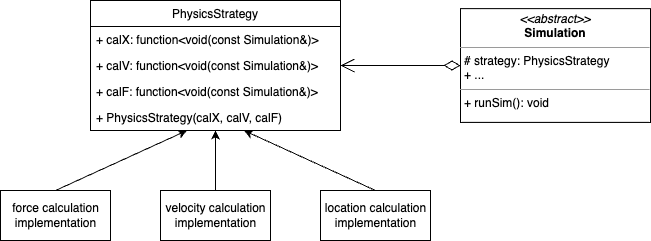
\includegraphics[width=\textwidth]{res/strategy.png}
        \caption{UML-like diagram showing our idea behind the strategy pattern}
        \label{fig:strat}
    \end{figure}
    \item We also abstracted the \verb|FileWriter| class to be able to use different output types i.e. VKT and XYZ sofar
\end{itemize}

\subsection{Improving the force calculations}
\label{sec:Refactoring:forceimprovements}

\begin{itemize}
    \item We implemented a second strategy for calculating the forces in our simulation
    \item For this we use the simple identity $F_{i,j} = -F_{j,i}$
        \begin{equation}
            F_{i,j} = \frac{m_im_j}{(||x_i-x_j||_2)^3} (x_j - x_i) = \frac{m_jm_i}{(||x_j-x_i||_2)^3} \left(-1 \cdot \left(x_i - x_j\right)\right) = - F_{j,i} 
        \end{equation}
    \item This is implemented using the pairwise iterator mentioned in \ref{sec:Refactoring:ParticleContainer}
    \item Theoretically, this should yield a speedup of 2, as only half the number of calculations are necessary
    \item The values we measured can be seen in Table \ref{tab:speedup}. This is only a speedup of around 1.25
        \begin{table}[H]
            \centering
            \begin{tabular}{|l|l|l|l|l|}
            \hline
                & Time for $10^6$ iterations \\ \hline
            Naive & 31109ms                  \\ \hline
            V2    & 24881ms                  \\ \hline
            \end{tabular}
            \caption{Values measured for the two different force calculation strategies. One being the naive implementation, while the other utilizes $F_{1,2} = - F_{2,1}$. This yields a speedup of approx 1.25.}
            \label{tab:speedup}
        \end{table}
    \item To reproduce the numbers, simply run the test code for timing both approaches. It will load the \verb|sonne-eingabe.txt| file and run a force calculation for $10^6$ times
    \item Note that this will vary
\end{itemize}

\subsection{Testing}

\begin{itemize}
    \item Even though tests were not mandatory, we opted to integrate some basic test to check our implementation
    \item This was done using the \verb|gtest| testing library
    \item This is mainly focused on the \verb|ParticleContainer| class and its iterators
    \item But we also included a test for the two different approaches on calculating the forces as mentioned in \ref{sec:Refactoring:forceimprovements} and measuring the speedup
    \item To run the tests follow the README
\end{itemize}

\end{document}